There are several ways by which the replacement value of an asset can be specified in the exposure model. The different options are listed below:

\begin{itemize}
	\item Specify the aggregate value of each asset
	\item Specify the value per unit, and provide the number of units in each asset
	\item Specify the value per unit area, and provide the aggregate area of each asset
	\item Specify the value per unit area, specify the area per unit, and provide the number of units in each asset
\end{itemize}

This case tests the computation of the loss curve and average loss when the aggregate asset value is provided in the exposure model. The vulnerability function used is the same as in Case~1d and shown in Table~\ref{tab:vf-ln-tax1-nzcov}. The aggregate asset value in this case is $20,000$. Apart from the change in the exposed value, the calculation procedure remains the same as described in Case~1d.

The loss curve calculated using the implementation of the calculator in Julia is compared with that produced by OpenQuake in Figure~\ref{fig:lc-ebr-4a}.

\begin{figure}[htbp]
\centering
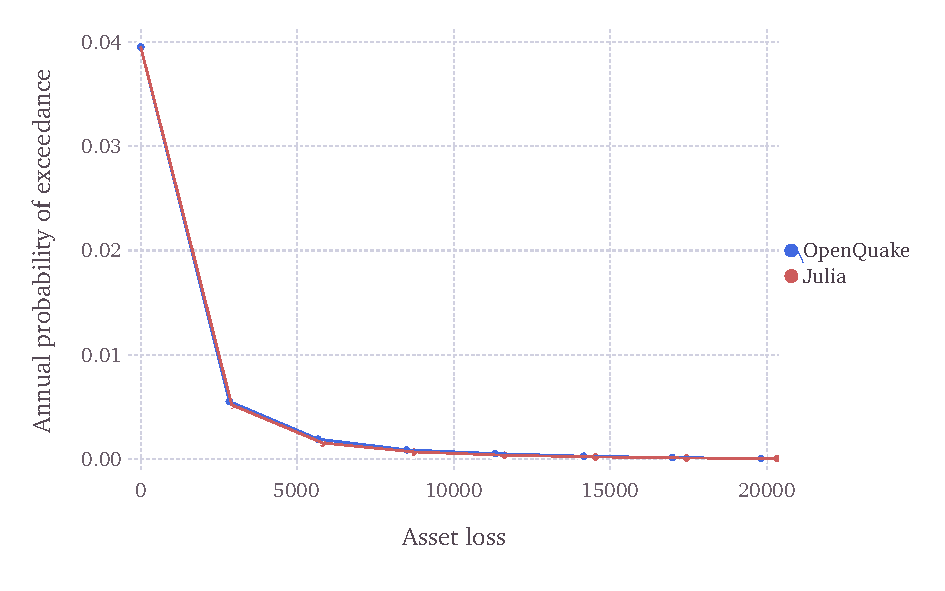
\includegraphics[width=12cm]{qareport/figures/fig-lc-ebr-4a}
\caption{Loss curve comparison for event based risk test case 4a}
\label{fig:lc-ebr-4a}
\end{figure}